\subsection{Anforderungen der Erklärungen}

Mithilfe der Rohanforderungen und Ziele aus dem Workshop sowie den erstellten Personas sowohl funktionale als auch nicht-funktionale Anforderungen für Erklärungen in NUNAV entwickelt werden

\subsubsection{Nicht-Funktionale Anforderungen}

% \cite{kohl_explainability_2019} gives a good overview to the requirement analysis for Explainability as an NFR

Als Methode zum Erstellen der konkreten NFRs wurde das Aufstellen eines Qualitätsmodells gewählt \cite{schneider2012abenteuer}. Das Modell ist in \autoref{fig:nunav_explanation_quality_model} abgebildet. Die allgemeinen Qualitätsziele sind in der Abbildung fett gedruckt und die Metriken kursiv dargestellt. Bei der Erstellung wurde immer iterativ Rücksprache mit den verschiedenen Teilnehmern des Workshops gehalten. Die Basis für die Qualitätsziele waren die in dem Modell für Erklärungen unter \textit{Objectives} aufgeführten Ziele. Die Endfassung der Anforderungen wurde schlussendlich vom Teamleiter des \glqq Mobile Application\grqq{}-Teams abgesegenet.

Es hat sich allerdings herausgestellt, dass das Aufstellen solch konkreter Anforderungen nicht der Arbeitsweise von Graphmasters entspricht. In den Rücksprachen wurde klar, dass die Ziele normalerweise deutlich abstrakter gehalten werden. Für eine Evaluation der Integration von Erklärungen im Rahmen dieser Arbeit werden die konkreten Anforderungen zur Prüfung allerdings benötigt.

\begin{figure}[htb!]
    \centering
    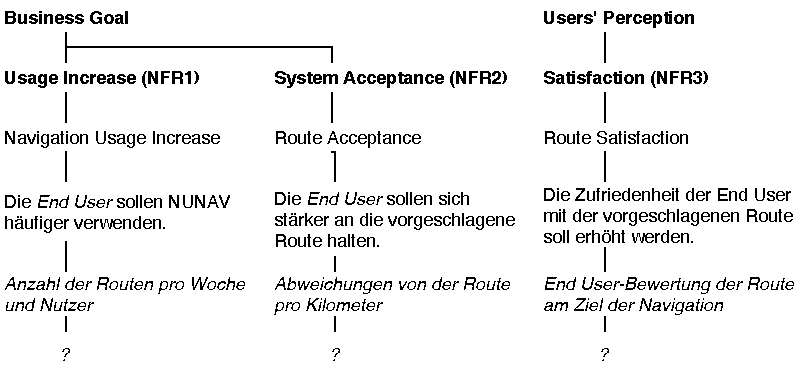
\includegraphics[width=\textwidth]{contents/06_model_evaluation/01_integration/res/quality_model.pdf}
    \caption{Qualitätsmodell für die Integration von Erklärungen in NUNAV Navigation}
    \label{fig:nunav_explanation_quality_model}
\end{figure}

In \autoref{fig:nunav_explanation_quality_model} ist zu erkennen, dass für Graphmasters im Allgemeinen die Erhöhung der Nutzung und die Akzeptanz des Systems im Fordergrund stehen. Für die Nutzung ist eigentlich die für Graphmasters interessanteste Metrik die Anzahl der aktiven Nutzer. Da für eine Messung von Veränderungen dieser durch die Integration von Erklärungen allerdings nicht über einen kurzen Zeitraum messen lässt, wurde  als Metrik die Anzahl der Routen pro Nutzer und Woche vorgeschlagen und schließlich auch durch Graphmasters bestätigt. Für die Akzeptanz des Systems ist ein Ziel, dass sich die \textit{End User} möglichst viel an die vorgeschlagene Route halten. Als Metrik wurde hierfür die Anzahl der Abweichungen von der Route pro Kilometer vorgeschlagen und ebenfalls letztendlich verwendet.

Ein weiteres wichtiges Ziel von Graphmasters ist die Zufriedenheit der \textit{End User} mit den Routen. Hierfür bestand bereits vor dem Beginn dieser Arbeit eine Metrik. \textit{End User} können bei Erreichen des Ziels einer Navigation auf einer Skala mit fünf Sternen angeben, wie zufrieden sie insgesamt mit der Route waren. Bis dato wurde diese Metrik allerdings noch nicht systematisch ausgewertet.

Für alle Metriken fällt auf, dass in \autoref{fig:nunav_explanation_quality_model} keine Sollwerte definiert sind. Aus den Gesprächen hat sich ergeben, dass für Graphmasters erstens nicht wichtig ist, um wie viel die verschiedenen Metriken sich verbessern, solange dies besser ist. Außerdem ist sind keine Basiswerte vorhanden, auf die man sich beziehen kann. Aus diesem Grund wurden die konkreten Anforderungen in Bezug auf signifikante Unterschiede formuliert. Die Formulierungen orientieren sich dabei an gängigen Vorlagen, enthalten allerdings nicht die, in den Vorlagen formulierten Sollwerte \cite{rajnish2010quality, wiegers1999writing, alexander2002writing}:

\begin{enumerate}
    \item [NFR1] Die Anzahl der gefahrenen Routen mit NUNAV pro Nutzer und Woche soll signifikant messbar erhöht werden.
    \item [NFR2] Die durchschnittliche Anzahl der Abweichungen der Nutzer pro Kilometer von der durch NUNAV vorgeschlagenen Route soll signifikant messbar verkleinert werden.
    \item [NFR3] Die durchschnittliche Bewertung der Route am Ende der Navigation in NUNAV soll signifikant erhöht werden.
\end{enumerate}

\subsubsection{Funktionale Anforderungen}

Für die Konkretisierung der funktionalen Anforderungen wurden auf die im Modell für Erklärungen vorgeschlagenen Ziele für Erklärungen betrachtet (\textit{Explanation Goals}). Außerdem wurde zur Lösung der Ziele der Katalog für Zusammenhänge der Erklärungen betrachtet, um positive Auswirkungen durch die Erklärungen auf die Ziele zu erreichen. Dabei steht vor allem auch die Frage im Raum, welche Aspekte genau erklärt werden müssen \cite{kohl_explainability_2019}.

Im durchgeführten Workshop wurden die Verständnisprobleme der Nutzer priorisiert und mit ersten Umsetzungsideen zusammengebracht. Aus diesen können die beiden Ziele \textit{Transparency} und \textit{Scrutability} für die Erklärungen abgeleitet werden. Da die vorherigen Qualitätsanforderungen sehr Allgemein auf \textit{NUNAV Navigation} bezogen sind, ist das Ziel, dass sich alle integrierten Erklärungen positiv auf die Qualitätsziele auswirken.

Auch die Konkretisierung der funktionalen Anforderungen ist iterativ erfolgt. Eine Herausforderung dabei war vor allem, dass Graphmasters sehr visuell arbeitet und statt genaue Anforderungen an neue Funktionen aufzustellen auf Basis von Ideen diese direkt als Prototypen oder Mockups umsetzt und diese dann iterativ weiterentwickelt.

Für die funktionalen Anforderungen wurde ein Zielbaum ähnlich zu Qualitätsmodellen aufgestellt, in dem die Konkretisierungsschritte zu sehen sind. \autoref{fig:nunav_explanation_functional_model} stellt diesen dar.

\begin{figure}[htb!]
    \centering
    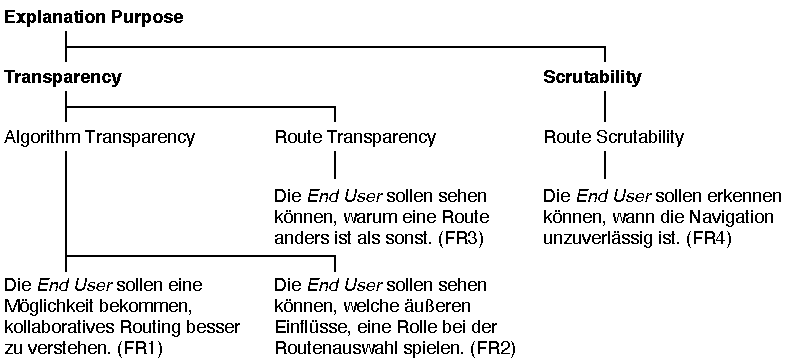
\includegraphics[]{contents/06_model_evaluation/01_integration/res/functional_model.pdf}
    \caption{Konkretisierungsschritte der funktionalen Anforderungen}
    \label{fig:nunav_explanation_functional_model}
\end{figure}

Aus den Konkretisierungsschritten (siehe \autoref{fig:nunav_explanation_functional_model}) wurden schlussendlich folgende funktionalen Anforderungen abgeleitet:
% . Die in der Abbildung als FR1 abgebildete unkonkrete Anforderung wurde im letzten Konkretisierungsschritt in zwei Anfroderungen (FR1.1, FR1.2) aufgeteilt.

\begin{enumerate}
    \item [FR1] NUNAV muss den \textit{End Usern} die Möglichkeit bieten, auf eine Erklärung zuzugreifen zu können, die den Routingalgorithmus erklärt.
    \item [FR2] NUNAV muss den \textit{End Usern} die Möglichkeit bieten, abzurufen, welche Informationen zu Verkehrsereignissen (z.B. Verkehrsfluss, Sperrungen, Baustellen, Staus) in den Algorithmus einfließen.
    \item [FR3] NUNAV muss den \textit{End Usern} während der Navigation Informationen zum Verkehrsgeschehen auf der aktuellen Route liefern.
    \item [FR4] Wenn die Genauigkeit der Positionierung unzuverlässig ist, den \textit{End Usern} dem Nutzer anzeigen, dass die Positionierung aktuell nicht zuverlässig ist.
\end{enumerate}

Auf Basis dieser Anforderungen wurden dann Erklärungen für die Integration in \textit{NUNAV Navigation} entwickelt.